\section{Setting up a hidden volume}

A TrueCrypt hidden volume exists within the free space of a typical
TrueCrypt volume. Given then the `outer volume' is accessed it is
(almost) impossible to determine if there is a hidden volume within it.
This is because TrueCrypt \emph{always} fills the empty space of an
encrypted volume with random data. So a hidden volume looks the same as
an empty TrueCrypt volume.

To create and use a hidden volume you need two passwords - one each for
the outer and inner (hidden) volumes. When you mount (open) the volume
you can use either password and that will determine which of the two is
opened. If you want to open just the hidden volume you use one password,
and if you want to access just the non-hidden encrypted volume you use
the other password.

To create a hidden volume open TrueCrypt and press the `Create Volume'
button:

\begin{figure}[htbp]
\centering
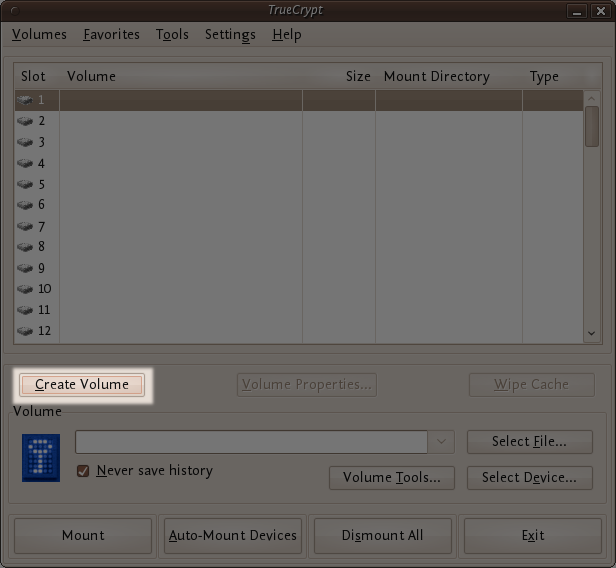
\includegraphics{hidden_vol_001.png}
\caption{Hidden volumes}
\end{figure}

The options for half of this process are almost the same as for setting
up a standard TrueCrypt volume and then the process continues for
setting up the hidden volume but lets go through the entire process step
by step anyway. In the screen shown below you just want to stay with the
default setting `Create an encrypted file container':

\begin{figure}[htbp]
\centering
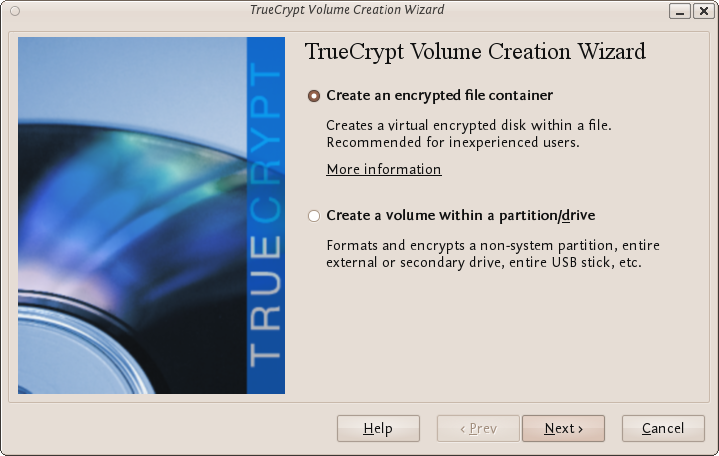
\includegraphics{hidden_vol_002.png}
\caption{Hidden volumes}
\end{figure}

Press `Next \textgreater{}' and continue to the next screen.

In the above screen you want to be sure that you choose the second
option `Hidden TrueCrypt Volume'. Select this and click on `Next
\textgreater{}' you will then be asked to choose the location and name
of the TrueCrypt \emph{outer} volume.

Click `Select File\ldots{}' and browse to a location for a new TrueCrypt
volume. We will use the name `myencryptedfile' in this example. Its the
same name as we used in the last example so be aware that if you have
just followed those instructions you must now create a new volume with a
new name.

\begin{figure}[htbp]
\centering
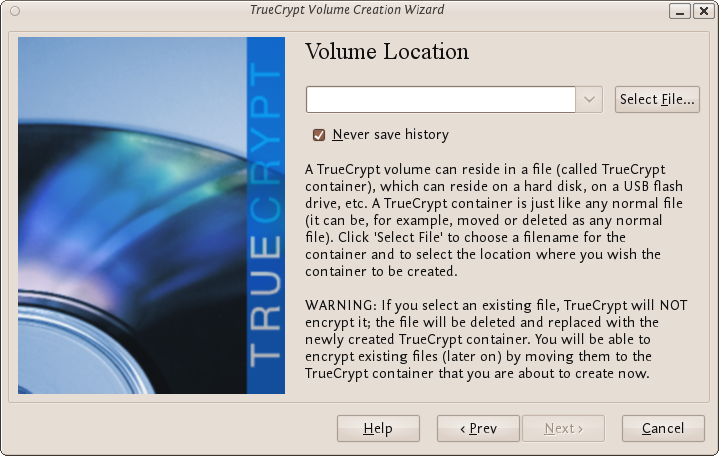
\includegraphics{hidden_vol_004.png}
\caption{Hidden volumes}
\end{figure}

Browse to the directory where you want to put the outer volume and enter
the name of the volume in the field named `Name' as in the example
above. When you are satisfied all is well click on `Save'. The file
browser will close and you return to the Wizard. Click `Next
\textgreater{}'. Here you are presented with some very technical
choices. Don't worry about them. Leave them at the defaults and click
`Next \textgreater{}'. The next screen asks you to determine the size of
the outer volume. Note that when you do this the maximum inner `hidden'
volume size is determined by TrueCrypt. This maximum size will of course
be smaller that the size you are setting on this screen. If you are not
sure what the ratio of outer volume size to inner (hidden) volume size
is then go through the process now as a `dummy' run - you can always
trash the encrypted volume and start again (no harm done).

So choose the size of the outer volume, I will choose 20MB as shown
below:

\begin{figure}[htbp]
\centering
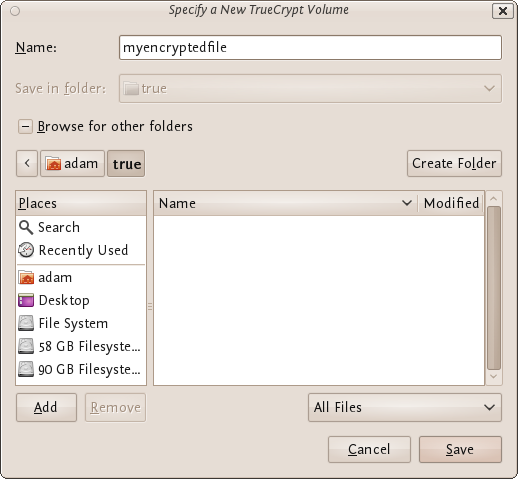
\includegraphics{hidden_vol_005.png}
\caption{Hidden volumes}
\end{figure}

You cannot set the outer volume size to be larger than the amount of
free space you have available on your disk. TrueCrypt tells you the
maximum possible size in bold letters so create a volume size smaller
than that. Then click `Next \textgreater{}' and you will be taken to a
screen asking you to set a password for the outer (not the hidden, this
comes later) volume.

\begin{figure}[htbp]
\centering
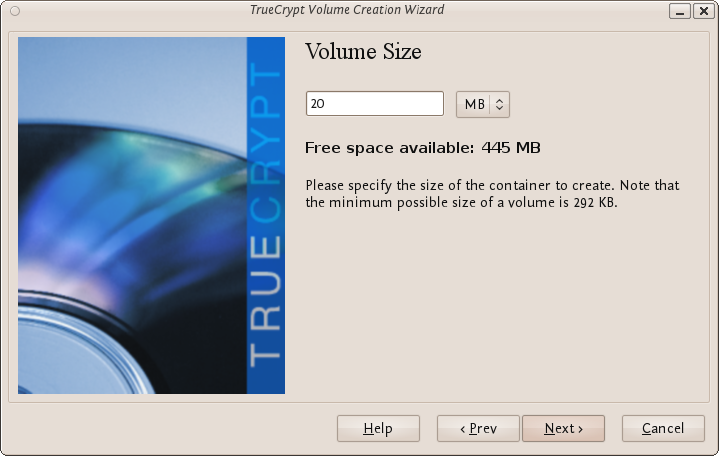
\includegraphics{hidden_vol_006.png}
\caption{Hidden volumes}
\end{figure}

Enter a password that is strong (see the chapter on creating good
passwords) and press `Next \textgreater{}'. Next TrueCrypt wants you to
help it create the random data it will fill the volume up with. So wave
your mouse around, browse the web, and do whatever you want for as long
as you can. When you feel TrueCrypt should be happy then press `Format'.
You will see a progress bar zip by and then you will be presented with
the next screen:

You can open the outer volume if you like but for this chapter we will
skip that and go ahead to create the hidden volume. Press `Next
\textgreater{}' and TrueCrypt will work out how the maximum possible
size of the hidden volume.

When you see the above screen just press `Next \textgreater{}'. Now you
must choose the encryption type for the hidden volume. Leave it at the
defaults and press `Next \textgreater{}'.

Now you will be asked to choose the size of the hidden volume.

I have set (as you see above) the maximum size as 10MB. When you have
set your maximum size press `Next \textgreater{}' and you will be
promoted to create a password for the hidden volume.

When creating the password for the hidden volume make sure you make it
substantially different fro the password for the outer volume. If
someone really does access your drive and finds out the password for the
outer volume they might try variations on this password to see if there
is also a hidden volume. So make sure the two passwords are not alike.

Enter your password in the two fields and press `Next \textgreater{}'.

Leave this window at the defaults and press `Next \textgreater{}' and
you will be presented with the same screen you have seen before to
generate random data for TrueCrypt. When you are happy click `Format'
and you should see the following :

\begin{figure}[htbp]
\centering
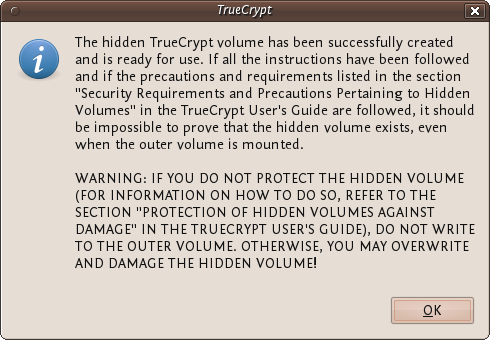
\includegraphics{hidden_vol_014.png}
\caption{Hidden volumes}
\end{figure}

The TrueCrypt manual it is referring to is not this manual. They mean
this manual : http://www.truecrypt.org/docs/

Click `OK' and keep and exit TrueCrypt. You can now mount the volume as
noted in the previous chapter.
